% THIS TEMPLATE IS A WORK IN PROGRESS

\documentclass{article}
\usepackage{graphicx}
\usepackage{hyperref}
\usepackage{fancyhdr}
\usepackage{float}

% FOR CODE
\usepackage{listings}
\usepackage{xcolor}

\definecolor{codegreen}{rgb}{0,0.6,0}
\definecolor{codegray}{rgb}{0.5,0.5,0.5}
\definecolor{codepurple}{rgb}{0.58,0,0.82}
\definecolor{backcolour}{rgb}{0.95,0.95,0.92}

\lstdefinestyle{mystyle}{
    backgroundcolor=\color{backcolour},   
    commentstyle=\color{codegreen},
    keywordstyle=\color{magenta},
    numberstyle=\tiny\color{codegray},
    stringstyle=\color{codepurple},
    basicstyle=\ttfamily\footnotesize,
    breakatwhitespace=false,         
    breaklines=true,                 
    captionpos=b,                    
    keepspaces=true,                 
    numbers=left,                    
    numbersep=5pt,                  
    showspaces=false,                
    showstringspaces=false,
    showtabs=false,                  
    tabsize=2
}

\lstset{style=mystyle}
% 

\fancypagestyle{firstpage}{%
  \lhead{CAP6610 Home Work 2}
  \rhead{Akash Gajjar}
}

\begin{document}
\thispagestyle{firstpage}

\section*{Question 1 Answer}

For a boolean function on 5 variables, the Karnaugh map has 32 cells, corresponding to the $2^{5} = 32$ possible input combinations. Each cell can be either 0 or 1, so there are $2^{32}$ possible boolean functions on 5 variables.

The maximum number of minterms in the Karnaugh map of a boolean function on 5 variables is 16. This is because if a boolean function on 5 variables has more than 16 minterms (i.e., more than 16 ones in its Karnaugh map), then at least one pair of adjacent cells can be grouped together to form a larger group of multiple cells that can be covered by a single gate. Therefore, the maximum number of gates required in a single hidden layer to implement a boolean function with 5 inputs is 16.

However, it's worth noting that constructing a network with 16 gates that can implement a complex function can be difficult in practice, and a more efficient network may require fewer gates. Increasing the number of layers in the network can allow for a more efficient implementation of the function. By adding additional layers to the network, the gates in each layer can be used to combine the output of gates in the previous layer, creating a hierarchical structure that can represent more complex functions with fewer gates. Any boolean function on $n$ variables can be expressed as a composition of boolean functions on two variables using the Boolean Algebra. We can construct the network like a binary tree, that would result in a tree with total 4 nodes and $\log_{2} 5 \approx 3$ layers. This is what the network would look like 

\begin{figure}[H]
  \centering
  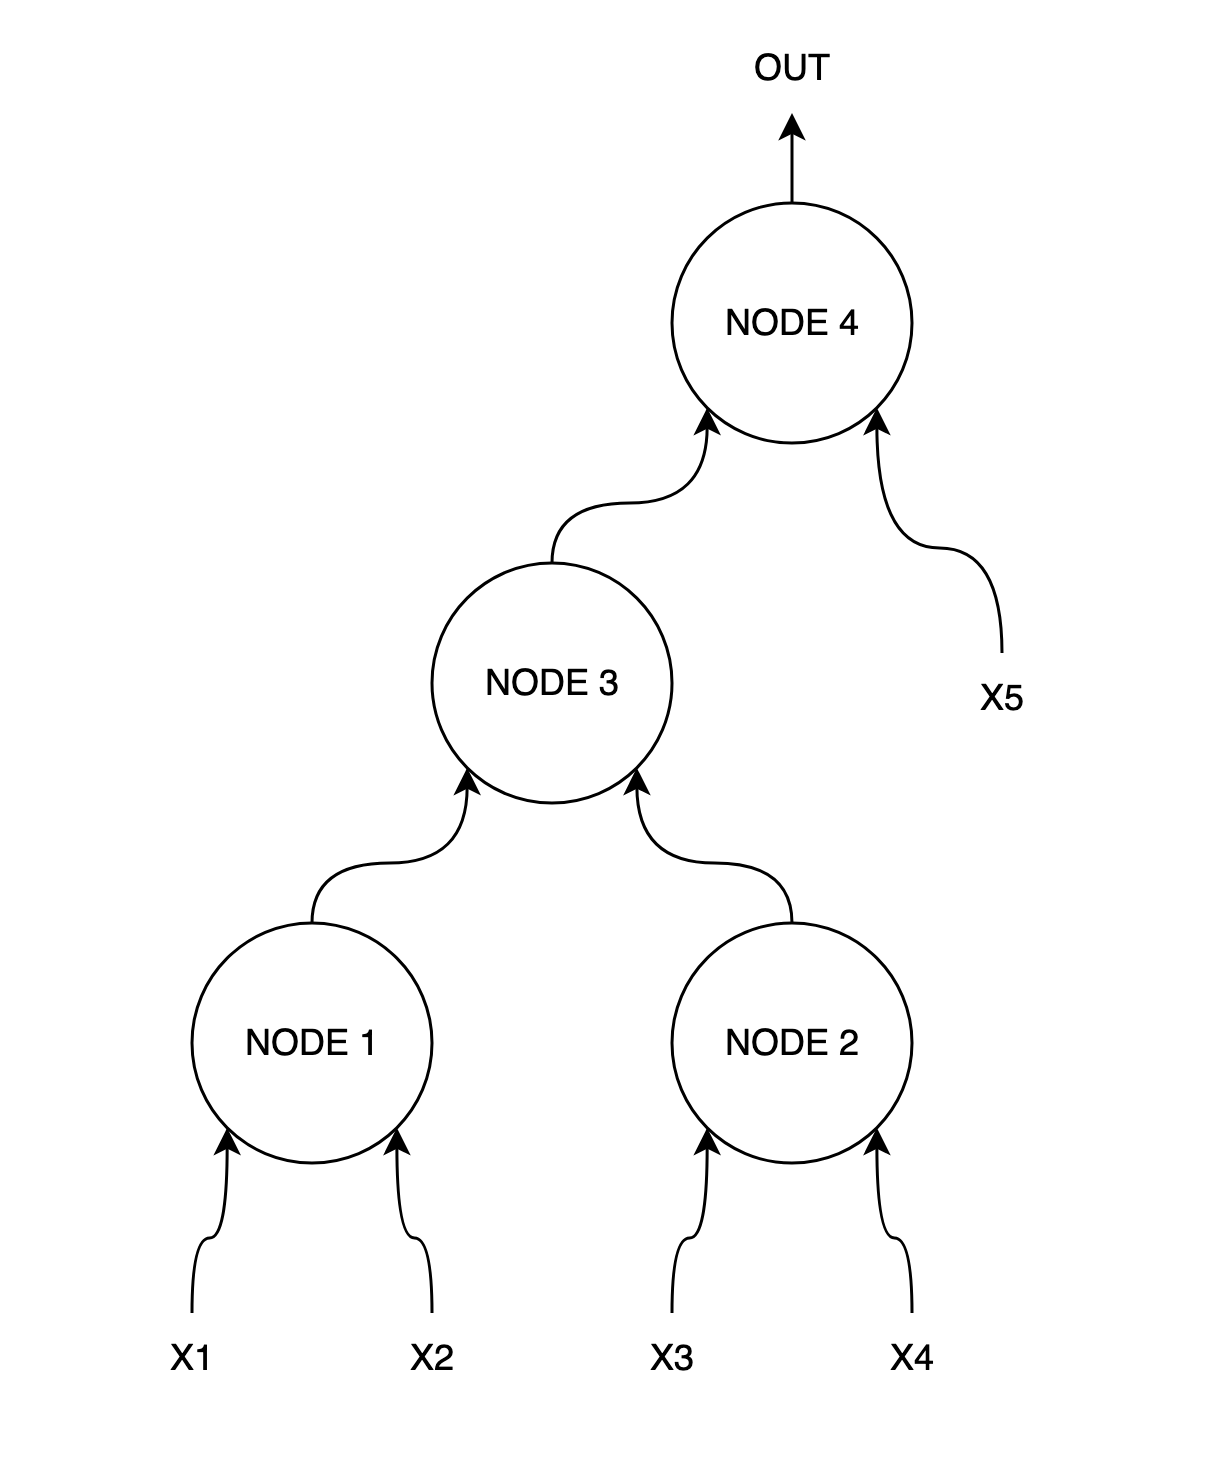
\includegraphics[width=2.5in]{images/network.png}
\end{figure}

Depending on the boolean function, there may be a case where the K-map reduces the whole function to a single gate.

\section*{Question 2 Answer}

\end{document}
